\section*{WRITING TASK 1}
You should spend about 20 minutes on this task.

\begin{quote}\large The plans show a neighbourhood square in Bellford in 2000 and after redevelopment in 2025.
\end{quote}
Describe the main features of the information, select relevant details, and make comparisons where appropriate.

\begin{center}
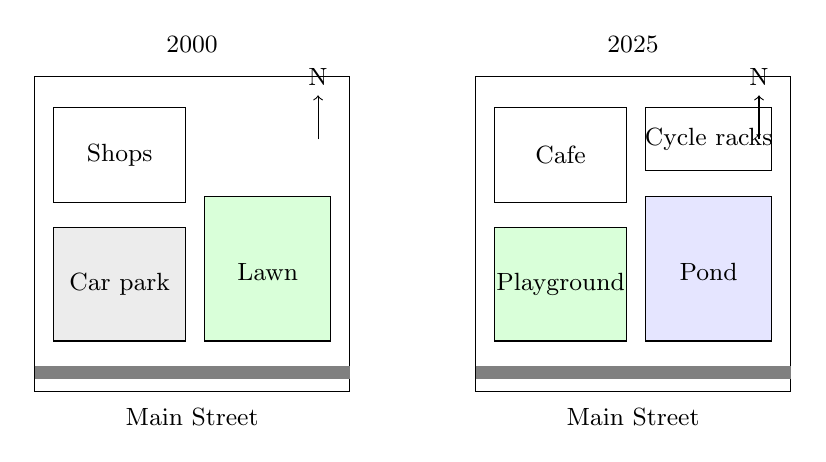
\begin{tikzpicture}[x=0.8cm,y=0.8cm,every node/.style={font=\small,align=center}]
\foreach \x/\year in {0/2000,7/2025}{\draw (\x,0) rectangle +(5,5);\node at (\x+2.5,5.5){\year};\draw[gray,line width=5pt] (\x,0.3)--+(5,0);\node at (\x+2.5,-0.4){Main Street};\draw[->] (\x+4.5,4)--+(0,0.7) node[above]{N};}
\draw[fill=gray!15] (0.3,0.8) rectangle (2.4,2.6);\node at (1.35,1.7){Car park};
\draw[fill=green!15] (2.7,0.8) rectangle (4.7,3.1);\node at (3.7,1.9){Lawn};
\draw (0.3,3) rectangle (2.4,4.5);\node at (1.35,3.75){Shops};
\draw[fill=green!15] (7.3,0.8) rectangle (9.4,2.6);\node at (8.35,1.7){Playground};
\draw[fill=blue!10] (9.7,0.8) rectangle (11.7,3.1);\node at (10.7,1.9){Pond};
\draw (7.3,3) rectangle (9.4,4.5);\node at (8.35,3.75){Cafe};\draw (9.7,3.5) rectangle (11.7,4.5);\node at (10.7,4){Cycle racks};
\end{tikzpicture}
\end{center}
Write at least 150 words.
\par\bigskip
{\footnotesize\color{gray} Original practice material; fictional settings and data. Not an official IELTS examination paper.}
